17. $\cfrac{2x^2+3x-13}{(x+3)(x-2)}>2\Leftrightarrow\cfrac{2x^2+3x-13-2x^2+4x-6x+12}{(x+3)(x-2)}>0\Leftrightarrow \cfrac{x-1}{(x+3)(x-2)}>0.$
Применив метод интервалов, найдём ответ: $x\in(-3;1)\cup(2;+\infty).$
\begin{figure}[ht!]
\center{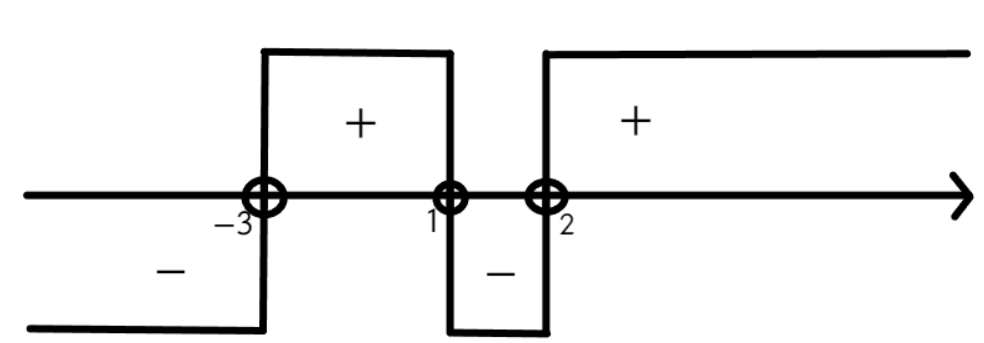
\includegraphics[scale=0.35]{ner9-17.png}}
\end{figure}\\
